\documentclass[11pt]{article}


%%%%%%%%%%%%%%%
\def\Type{ApplicationDJ}
\def\TypeNum{During-class for Application Day: Gradient Descent Method}
\def\TypeTitle{Gradient Descent}
\def\Semester{Fall 2025}
\def\Course{Math 1190/1210}
%\def\Targets{{\bf\color{Goldenrod}AD1}}
\def\desmosClassCode{{\bf ZAJ$3$AZ}}
\usepackage{preambleDJ}
\usepackage{graphicx}
\usepackage{footnote}
\usepackage{tikz}
\usepackage{pgfplots}
\usepackage[colorlinks=true, linkcolor=blue, urlcolor=blue]{hyperref}
%\pgfplotsset{compat=1.18}  % adjust to your version
\makesavenoteenv{minipage}
\begin{document}
%!TEX TS-program = xelatex
%!TEX encoding = UTF-8 Unicode



\pagestyle{otherpages}
\thispagestyle{firstpage}
\vspace*{.65in}


%!TEX TS-program = xelatex
%!TEX encoding = UTF-8 Unicode



%If Ada Lovelace\footnote{\url{https://en.wikipedia.org/wiki/Ada_Lovelace}} is the ``mother of programming" then 
{\bf Introduction}\\

\noindent
\begin{minipage}[c]{0.35\textwidth}
    \centering
    
\includegraphics[width=\linewidth]{Spring 2026/ApplicationDays/GradientDescent/images/feiFeiLiWiredCropped.png}
    Fei-Fei Li is known as the ``godmother of A.I'' for her groundbreaking contributions in computer vision and deep learning and as the creator of ImageNet\footnote{
See ``Godmother of A.I." Fei-Fei Li on technology development: ``The power lies within people" at \url{https://www.cbsnews.com/news/godmother-of-a-i-on-technology-development-fei-fei-li/}\\
or Britannica at \url{https://www.britannica.com/biography/Fei-Fei-Li}, The Guardian \href{https://www.theguardian.com/technology/2023/nov/05/ai-pioneer-fei-fei-li-im-more-concerned-about-the-risks-that-are-here-and-now}{\underline{here}} or \url{https://en.wikipedia.org/wiki/Fei-Fei_Li}
}.
\end{minipage}
\hspace{0.02\textwidth}
\begin{minipage}[c]{0.63\textwidth}


\vspace{1em}

In this application, we will be exploring how the tools of calculus can be applied in machine learning. \textit{Machine learning} refers to computer programs for which the outputs mimic patterns in a specific dataset, but without these patterns being explicitly described in the programming. This field powers much of modern artificial intelligence. For example, while generative AI's like ChatGPT can produce coherent English sentences, their code does not contain the rules of English grammar and syntax; rather, they ``learn" these rules autonomously by processing large amounts of examples. 

This learning process can be viewed as an optimization problem in the following way:
\begin{itemize}
    \item The algorithm to generate new outputs contains many \textit{parameters,} which each influence the outputs generated.
    \item Once the parameters have been chosen, the outputs of the algorithm are compared against the data set. The algorithm is then given a \textit{loss} score, where a smaller loss indicates a closer match to the data.
    \item The \textit{loss function} takes the parameters as input and gives the loss of the corresponding algorithm as an output. The optimization problem is then to find the parameter set which minimizes the loss function.
\end{itemize}
\end{minipage}
\newpage


















%%%%%%%%%%%%%%%%%%%%%%%%%%%%%%%%%%%%%%%%%%%%%%%%%%%%%%%%%%%%%%%%%%%%%%%%%%%%%%%%%%%%%%%%%%%%%%%%%%%%%%%%%%%%%%%%%%%%%%%%%%%%%%%%%%%%%%%%%%%%%%%%%%%%%%%%%%%%%%%%%%%%%%%%%%%%%%%%%%%%%%%%%%%%%%%%%%%%%%%%%%%%%%%%%%%%%%%%%%%%

Unfortunately, this optimization problem is usually much harder than the ones we've seen in this class so far. One big difference is the number of inputs: every function we've seen has had just one input $x$, while machine learning models can have billions of parameters or more. This means it is very hard to visualize or graph the loss function. Another issue is that the function itself is so complicated that we cannot simply write down the derivative and find critical numbers in the usual way.

In this situation, one of the tools we can use is \textit{gradient descent}. Gradient descent is a method used for optimization which only requires us to be able to evaluate a function and its derivative at individual points in the domain. Throughout this worksheet, we will develop the ideas of gradient descent for a single-variable function $f(x)$.

{\bf Example 1: Function and Derivative}\\

Suppose that we evaluate our function and its derivative at $x=1$ to get that $f(1) = 1$ and $f'(1) = 2$.

\begin{enumerate}
\item Write down the equation of the line tangent to $f(x)$ at the point $(1,1)$:
\[
    y = \underline{{\color{blue}y = 2x  -1}}
\]
\end{enumerate}

A small segment of the tangent line is sketched below in red, along with an example in blue of what $f(x)$ might look like near the point $(1,1)$.

\begin{center}
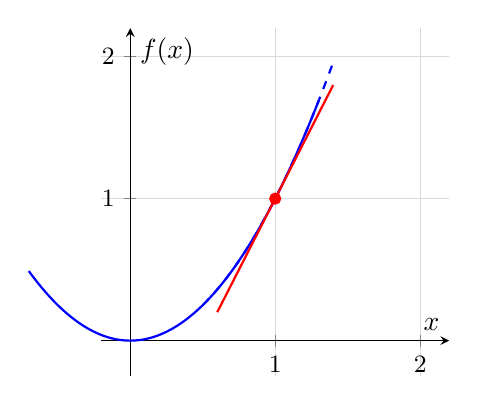
\begin{tikzpicture}
\begin{axis}[
    height = 6cm,
    width = 6cm,
    axis lines=middle,
    xlabel=$x$, ylabel=$f(x)$,
    xmin=-0.2, xmax=2.2,
    ymin=-0.25, ymax=2.2,
    xtick={0,1,2},
    ytick={0,1,2},
    grid=both,              % add grid lines
    grid style={gray!30},   % light gray grid
    tick label style={font=\small}, % smaller labels
    enlargelimits=false,
    clip=false
]

% f(x) = x^2
\addplot [domain=-0.7:1.3, samples=100, blue, thick] {x^2};
\addplot [domain=0.5:1.4, samples=100, blue, thick, dashed] {x^2};

% Tangent at x=3: f'(3) = 6
\addplot [domain=0.6:1.4, red, thick] {2*(x-1)+1};

% Mark the point (3,9)
\addplot[only marks, mark=*, red] coordinates {(1,1)};
% \node[below right] at (axis cs:1,1) {$(1,1)$};

\end{axis}
\end{tikzpicture}
\end{center}

Call the $x$-value we're currently examining $x_1=1$. We want to choose a new guess $x_2$ which is closer to the minimum of $f(x)$.
From this picture, we can see that since $f'(x_1)>0$, if we pick $x_2 < x_1$ then hopefully  $f(x_2)$ is closer to the minimum. But how much smaller should we make $x_2$? If we change our guess too much, we may overshoot the minimum, but if we change it too little we won't make much progress towards finding the minimum. 

The formula we will use to update our guess is this:
\[
    x_2 = x_1 - \alpha f'(x_1),
\]
where $\alpha$ is some positive constant.
\begin{enumerate}
    \item[2.]  Using $\alpha = 0.1$, compute $x_2$ in our example.
    \[
        x_2 = \underline{{\color{blue}1 - 0.1(2) = 0.8}}
    \]
\end{enumerate}
\newpage
This formula makes sense because:
\begin{itemize}
    \item If $f'(x_0)>0$, this moves our guess to the left, just like we wanted. If $f'(x_0) < 0$, this moves our guess to the right.
    \item If $f'(x_0)$ is close to zero, then we're probably close to the minimum and our guess won't move much. If $f'(x_0)$ is large, then the guess will change significantly.
    \item Adjusting the constant $\alpha$ allows us to fine-tune the gradient descent process, either speeding it up or making sure we don't overshoot the minimum.
\end{itemize}
We can then use $f'(x_2)$ to make a new guess $x_3$, use $f'(x_3)$ to make a new guess $x_4$, and so on and so forth until we are confident our guess is close to the minimum.
\begin{figure}[h!]
\centering
\begin{minipage}{0.45\textwidth}
\centering
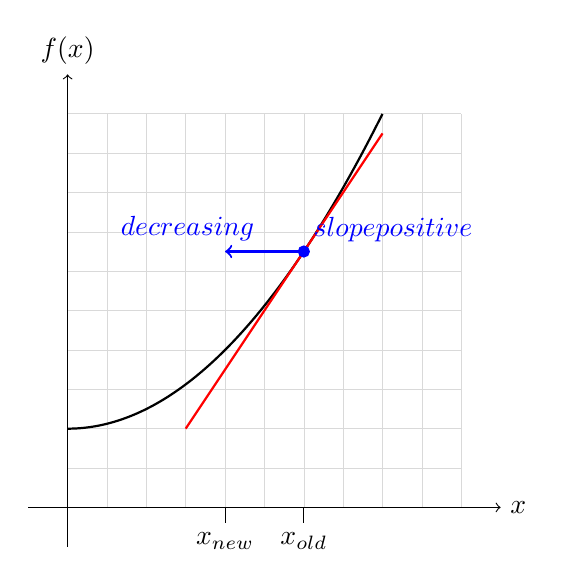
\begin{tikzpicture}[scale=1.0]
    % grid
    \draw[step=0.5, gray!30, very thin] (0,0) grid (5,5);
    
    % axes
    \draw[->] (-0.5,0) -- (5.5,0) node[right] {$x$};
    \draw[->] (0,-0.5) -- (0,5.5) node[above] {$f(x)$};
    
    % function
    \draw[thick, domain=0:4, samples=100, smooth] plot (\x,{0.25*\x*\x+1});
    
    % tangent line through x=3
    \draw[red, thick, domain=1.5:4] plot (\x,{1.5*\x -1.25}); % tangent using slope f'(3)=3
    
    % point on curve
    \filldraw[blue] (3,3.25) circle (2pt) node[above right] {$\text{slope positive}$};
    
    % gradient descent arrow
    \draw[->, thick, blue] (3,3.25) -- (2,3.25) node[midway, above left] {$\text{decreasing }$};
    
    % x labels
    \draw (3,0) -- (3,-0.2) node[below] {$x_\text{old}$};
    \draw (2,0) -- (2,-0.2) node[below] {$x_\text{new}$};
\end{tikzpicture}
\caption*{Slope $f'(x_\text{old})>0$: move left along $x$ to decrease $f(x)$.}
\end{minipage}
\hfill
\begin{minipage}{0.45\textwidth}
\centering
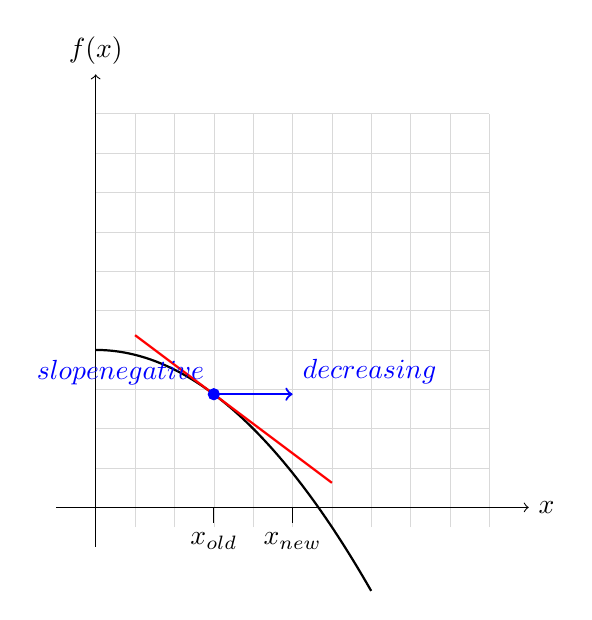
\begin{tikzpicture}[scale=1.0]
    % grid
    \draw[step=0.5, gray!30, very thin] (0,-0.25) grid (5,5);
    
    % axes
    \draw[->] (-0.5,0) -- (5.5,0) node[right] {$x$};
    \draw[->] (0,-0.5) -- (0,5.5) node[above] {$f(x)$};
    
    % function
    \draw[thick, domain=0:3.5, samples=100, smooth] plot (\x,{-0.25*\x*\x+2});
    
    % tangent line through x=1.5
    \draw[red, thick, domain=0.5:3] plot (\x,{-0.75*\x + 2.5625}); % tangent f'(1.5)=1.5
    
    % point on curve
    \filldraw[blue] (1.5,1.4375) circle (2pt) node[above left] {$\text{slope negative}$};
    
    % gradient descent arrow
    \draw[->, thick, blue] (1.5,1.4375) -- (2.5,1.4375) node[above right] {$\text{decreasing}$};
    
    % x labels
    \draw (1.5,0) -- (1.5,-0.2) node[below] {$x_\text{old}$};
    \draw (2.5,0) -- (2.5,-0.2) node[below] {$x_\text{new}$};
\end{tikzpicture}
\caption*{Slope $f'(x_\text{old})<0$: move right along $x$ to decrease $f(x)$.}
\end{minipage}
\end{figure}

\newpage
{\bf Gradient Descent Algorithm}\\

\enum{

\item Let's apply gradient descent to $f(x) = x^4 - 2x^2 + 1$ with $x_1 = 2$ and $\alpha = 0.02$. You may need a calculator.

\enum{
\item Compute $f'(x)$.
\underline{{\color{blue} $4x^3 - 4x$}}
\item Evaluate $f'(x_1)$, and use this to compute a new guess $x_2$.
{\color{blue}$f'(x_1) = f'(2) =   4(2)^3 - 4(2) = 24$
So, $$x_2 = x_1 - \alpha f'(x_1) = 2 - 0.02(24) = 1.52$$
}
\item Evaluate $f'(x_2)$, and use this to compute a new guess $x_3$.
{\color{blue}$f'(x_2) = f'(1.52) =   4(1.52)^3 - 4(1.52) = 7.97$
So, $$x_3 = x_2 - \alpha f'(x_2) = 1.52 - 0.02(7.97) = 1.36$$
}\item Using our usual optimization tools, where are the local minima of $f(x)$? Which minimum, if any, do our guesses seem to be approaching?
{\color{blue} $f'(x) = 4x^3 - 4x$
and $f'(x) = 0 \iff 4x^3 - 4x = 0 \iff x(4x^2 - 4) = 0 \iff x = 0 \text{ or } x = \pm 1$.
$f''(x) = 12x^2 - 4$
and $f''(\pm 1) = 8 > 0$ and $f''(0) = -4  <  0$ So, we have a local max at $x = 0$ and local mins at $x = \pm 1$
Our guesses seem to be approaching the local minimum at $x = 1$.
}
}
}

\newpage
\section*{Gradient Descent Exploration Activity}

Now open the Gradient Descent app found here: \href{https://woodword0-gradientdescentapplication.hf.space/}{Open the Gradient Descent App}


\begin{itemize}
    \item Select a function from the drop down menu
    \item Try different starting points $x_0$
    \item Try different learning rates $\alpha$
    \item Observe the sequence of points
\end{itemize}

\textbf{Answer the following questions:}

\begin{enumerate}

    \item For $f(x) = x^2$:
    \begin{itemize}
        \item Does gradient descent always find the minimum?
         {\color{blue}
         No. The process is very dependent on the choice of starting point, the choice of $\alpha$ and the number of steps. Sometimes it gets very close to the minimum and other times it does not.
         }
        
        \item What happens if $\alpha$ is very large?
    \end{itemize}
  {\color{blue}
        When the learning rate in gradient descent is too large, the iterates fail to converge smoothly to a local minimum and instead oscillate around it. 
Consider gradient descent:
\[
x_{k+1} = x_k - \alpha f'(x_k),
\]
and assume \(x^*\) is a local minimum. 
If \(1 - \alpha \lambda < 0\), the sign of the error alternates each iteration, causing the iterates to overshoot the minimum and oscillate. When \(|1 - \alpha \lambda| \ge 1\), the method fails to converge, leading either to sustained oscillations or divergence.
    }

    \item For $f(x) = e^x - x$:
    \begin{itemize}
        \item Does the method converge to the same point from different starting values?
        {\color{blue} Yes. In this case, regardless of from where you choose the starting point, the  method converges to the single minimum value at $x = 0$ (as long as you choose a reasonable learning rate $\alpha$ and number of steps.}
        
        \item What do you notice about the slope near the minimum?
    \end{itemize}
    {\color{blue} The slope approaches zero as we approach the minimum. This can be seen from the following limit. $\displaystyle \lim_{x \to 0}f'(x) = \displaystyle \lim_{x \to 0}e^x - 1 = 0$}
    \item For $f(x) = x^4 - 2x^2 + 1$:
    \begin{itemize}
        \item How many minimums does this function have?
    {\color{blue} Using problem 1 (d), we can see that this function has two local minimums (at $x \pm 1$ and a local maximum at $x = 0$.
    }        
        \item Does gradient descent always find the same one?
         {\color{blue}
         No. This depends on the starting point.}
        
        \item How does the starting point affect the result?
        {\color{blue}
         The algorithm will converge to whichever minimum to which the starting point is closest, if the learning rate and number of steps are chosen appropriately (for example take $x_0 = -0.8$, $\alpha = 0.5$ and 30 steps). If the learning rate is too large, it may not converge to either minimum (for example take $x_0 = -0.82$, $\alpha = 0.1$ and 30 steps), or you can start near one and make the algorthm converge to the other (for example take $x_0 = -0.82$, $\alpha = 0.5$ and 30 steps). }
    \end{itemize}

\end{enumerate}








%%%%%%%%%%%%%%%%%%%%%%%%%%%%%%%%%%%%%%%%%%%%%%%%%%%%%%%%%%%%%%%%%%%%%%%%%%%%%%%%%%%%%%%%%%%%%%%%%%%%%%%%%%%%%%%%%%%%%%%%%%%%%%%%%%%%%%%%%%%%%%%%%%%%%%%%%%%%%%%%%%%%%%%%%%%%%%%%%%%%%%%%%%%%%%%%%%%%%%%%%%%%%%%%%%%%%%%%%%%%

\section*{During Class Application: Estimating Disease Spread with Gradient Descent}
In this activity. we will use gradient descent on real-world corona virus data to model a parameter called $R_0$ - the expected number of new infections produced by a single (typical/average) infectious individual.
The base reproduction number, $R_0$, (also called the base reproductive ratio) is defined as the expected number of new infections produced by a single (typical/average) infectious individual, when introduced into a totally susceptible population. $R_0$ is used in epidemiological studies of infectious diseases to gauge how contagious/transmissible an infectious disease is: if $R_0 < 1$, the disease will die out, and if $R_0 > 1$ infection can increase in the population. It is also used to determine how effective vaccination or other disease mitigation strategies need to be in order to protect populations from infection.
During the early stages of a disease outbreak, the number of cases often follows an exponential model:



\[
I(t) = e^{\lambda t}
\]
We can use this as a prediction function for the number of cases.
Taking the natural logarithm of both sides gives:
\[
\ln (I(t)) = \lambda t
\]

This transforms the exponential model into a \textbf{linear model}:
\[
\hat{y}(t) = \lambda t
\]
where:
\begin{itemize}
    \item $t$ = time (days),
    \item $\hat{y}(t) = \ln (I(t)) = \lambda t$ = predicted log of observed number of cases, and the prediction function.
    \item $\lambda$ = growth rate (how fast the infectious disease is spreading - unknown parameter).
\end{itemize}
\vspace{1cm}

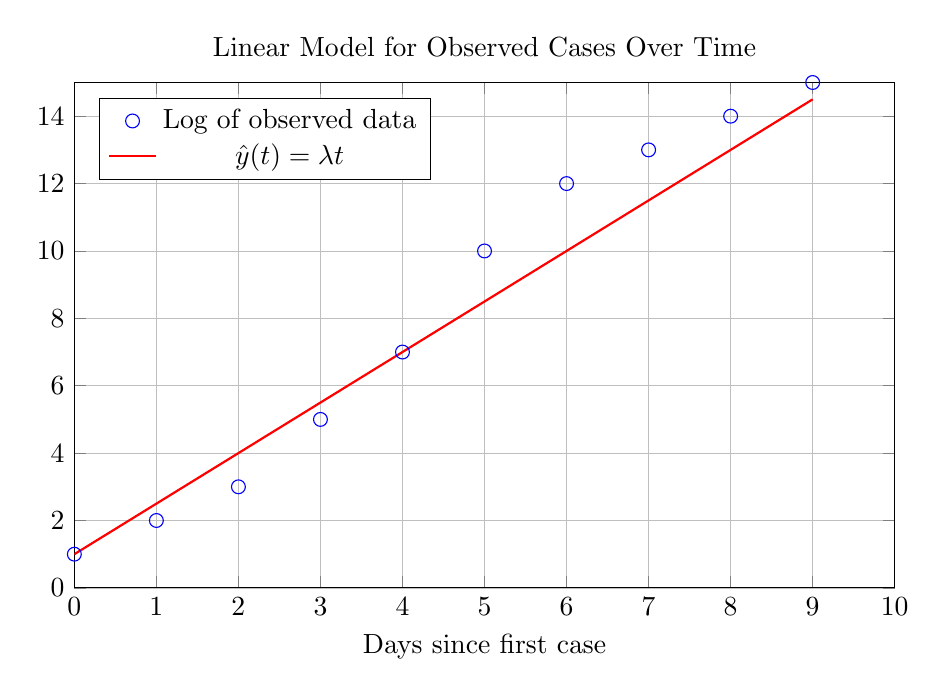
\begin{tikzpicture}
\begin{axis}[
    title={Linear Model for Observed Cases Over Time},
    xlabel={Days since first case},
  ylabel={},
  %$\log(\text{Number of Cases})$
    xmin=0, xmax=10,
    ymin=0, ymax=15,
    grid=both,
    major grid style={line width=.2pt,draw=gray!50},
    minor grid style={line width=.1pt,draw=gray!20},
    width=12cm,
    height=8cm,
    legend pos=north west,
]

% Data points
\addplot[
    only marks,
    mark=o,
    mark size=2.5pt,
    blue,
] coordinates {
    (0,1) (1,2) (2,3) (3,5) (4,7) (5,10) (6,12) (7,13) (8,14) (9,15)
};
\addlegendentry{Log of observed data}

% Line of best fit
\addplot[
    red,
    thick,
    domain=0:9,
] {1.5*x + 1};
\addlegendentry{$\hat{y}(t) = \lambda t$}

\end{axis}
\end{tikzpicture}

Our goal is to find the value of $\lambda$ that best fits the data.
\section*{Setting up Gradient Descent with a Single Data Point}
To start with, suppose we only have one data point $(t_0,y_0)$ of observed data.
%%%%%%%%%%%%%%%%%%%%%%%%%%%%%%%%%%%%%%%%%%%%%%%%%%%%%%%%%%%%%%%%%%%%%%%%%%%%%%%%%%%%%%%%%%%%%%%%%%%%%%%%%%%%%%%%%%%%%%%%%%%%%%%%%%%%%%%%%%%%%%%%%%%%%%%%%%%%%%%%%%%%%%%%%%%%%%%%%%%%%%%%%%%%%%%%%%%%%%%%%%%%%%%%%%%%%%%%%%%%
\begin{enumerate}

\item \textbf{Error Function with a Single data point}\\
%\textbf{The Initial Problem:} \\

We do not know the value of $\lambda$, but if we are given a single  data point consisting of two numbers $(t_1,\ln(I(t_1))) = (t_1,y_1)$,
we can use our gradient descent algorithm to try to find the value of $\lambda$ that makes our model match this data point. To do this we try to minimize the squared error between the data we have observed and our predictions:
\[
E(\lambda) = \big(y_1 - \lambda t_1\big)^2
\]
\item \textbf{Setting up gradient descent for a single data point.}\\
    We can now take the derivative with respect to our variable $\lambda$ of our error function $E(\lambda)$ using the chain rule.
  %      \begin{enumerate}
    To reduce the error, we:
    \begin{enumerate}
    \item[(a)] \textbf{Choose an initial guess} $\lambda_1 = \lambda_{\text{old}}$ for $\lambda$\\
    \item[(b)] \textbf{Compute a prediction} $\hat{y}_1(t_1) = \lambda_1 t_1$\\

    \item[(c)] \textbf{Compute the derivative} with respect to $\lambda$ of the error function:
    \[
    \frac{dE}{d \lambda} = 2\big(y_1 - \lambda t_1\big) \cdot (-t_1)
    \]
    \item[(d)] Then \textbf{update} $\lambda$ using:
    \[
    \lambda_{\text{new}} = \lambda_{\text{old}} - \alpha \cdot 2\big(y_1 + \lambda_{\text{old}}t_1\big)
    \]
    where $\alpha > 0$ is the \textbf{step size} (learning rate).
    \end{enumerate}
    \vspace{0.5cm}
    
Overall, the process can be defined as follows:\\
\vspace{0.5cm}\

\textbf{Summary}
\begin{itemize}
    \item Choose an initial guess $\lambda_1$ for $\lambda$\\
    \item Compute your predictions.
    \item Compute the derivative of the error function.\\
    \item Update $\lambda$ with gradient descent.
\end{itemize}
\end{enumerate}
%%%%%%%%%%%%%%%%%%%%%%%%%%%%%%%%%%%%%%%%%%%%%%%%%%%%%%%%%%%%%%%%%%%%%%%%%%%%%%%%%%%%%%%%%%%%%%%%%%%%%%%%%%%%%%%%%%%%%%%%%%%%%%%%%%%%%%%%%%%%%%%%%%%%%%%%%%%%%%%%%%%%%%%%%%%%%%%%%%%%%%%%%%%%%%%%%%%%%%%%%%%%%%%%%%%%%%%%%%%%
\newpage
\subsection*{You Try!}

Suppose we observe the the spread of the disease for just one day and found the following data:

\[
\begin{array}{c|c}
t_i & y_i = \ln I(t_i) \\
\hline
1 & 1 \\
\end{array}
\]
So our single data point is $(1,1)$ Let's use this data point to update gradient descent once.
\begin{enumerate}
\item[(a)] Choose an initial guess:
Let's assume
$\lambda_1 = 0.5, \quad \alpha = 0.1$\\
%\vspace{3cm}

\item[(b)] Compute a prediction:

$\hat{y}_1 = \lambda_1 t_1$ = {\color{blue}
 \underline{$\hat{y}_1 = \lambda t_1  = 0.5\cdot (1) = 0.5$}
 }
\\
\vspace{3cm}

 
\item[(c)] Compute derivative:
\(
\frac{dE}{d\lambda} = 2(y_1 - \hat{y}_1)(-t_1)
\)
{\color{blue}
\begin{align*}
    \frac{dE}{d\lambda} &= 2(y_1 - \hat{y}_1)(-t_1)\\
    &= 2(1 - \lambda_1 t_1)(-t_1)\\
    &= 2(1 - 0.5)(-1)\\
    &= 2(0.5)(-1)\\
    &= -1
\end{align*}
}
\item[(d)] Update:
$
\lambda_2 = \lambda_1 - \alpha \frac{dE}{d\lambda}$
= 
 {\color{blue}
 \underline{$\lambda_2 = \lambda_1 - \alpha \frac{dE}{d\lambda} = 0.5 - (0.1) \cdot (-1) = 0.6$}
 }
\end{enumerate}
%%%%%%%%%%%%%%%%%%%%%%%%%%%%%%%%%%%%%%%%%%%%%%%%%%%%%%%%%%%%%%%%%%%%%%%%%%%%%%%%%%%%%%%%%%%%%%%%%%%%%%%%%%%%%%%%%%%%%%%%%%%%%%%%%%%%%%%%%%%%%%%%%%%%%%%%%%%%%%%%%%%%%%%%%%%%%%%%%%%%%%%%%%%%%%%%%%%%%%%%%%%%%%%%%%%%%%%%%%%%
\newpage
\section*{Setting up Gradient Descent with several data points}
Now, suppose we have several data points $(t_1,y_1), (t_2,y_2) \ldots (t_{n},y_{n})$ of observed data.
It turns out that to get the error function we can just take an average over the squares of all of the errors; that is the differences between the observed values and the predicted values.
\vspace{1cm}

\begin{center}

\includegraphics[width=0.6\linewidth]{Spring 2026/ApplicationDays/GradientDescent/images/MeanSquaredError.png}
\end{center}

\begin{center}
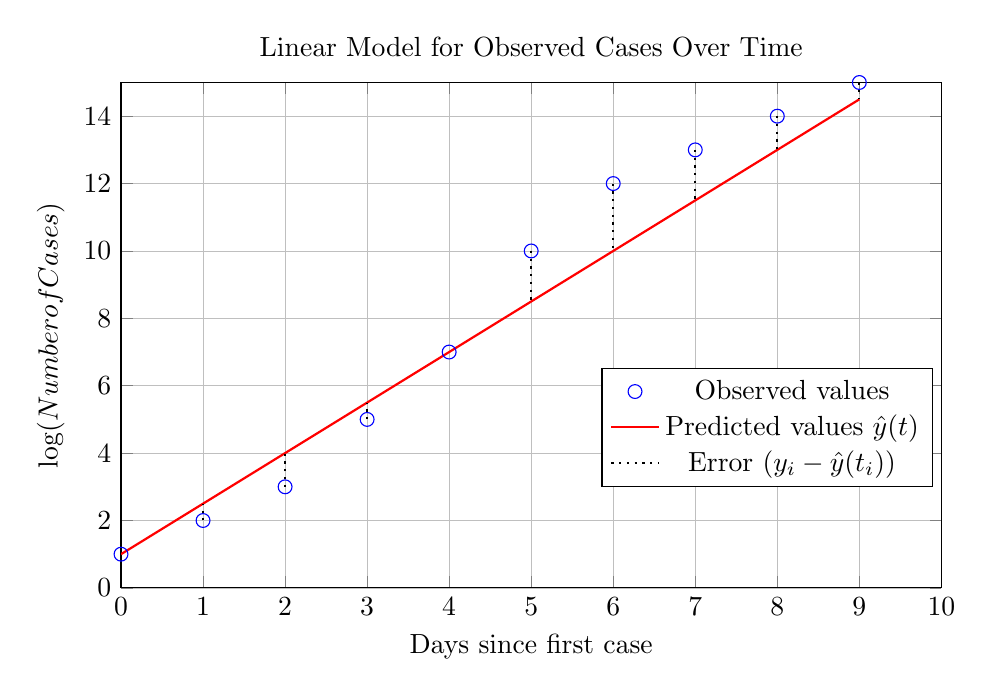
\begin{tikzpicture}
\begin{axis}[
    title={Linear Model for Observed Cases Over Time},
    xlabel={Days since first case},
    ylabel={$\log(\text{Number of Cases})$},
    xmin=0, xmax=10,
    ymin=0, ymax=15,
    grid=both,
    major grid style={line width=.2pt,draw=gray!50},
    minor grid style={line width=.1pt,draw=gray!20},
    width=12cm,
    height=8cm,
    legend style={
    at={(0.99,0.2)},
    anchor=south east
}
]

% Data points
\addplot[
    only marks,
    mark=o,
    mark size=2.5pt,
    blue,
] coordinates {
    (0,1) (1,2) (2,3) (3,5) (4,7) (5,10) (6,12) (7,13) (8,14) (9,15)
};
\addlegendentry{Observed values}

% Line of best fit
\addplot[
    red,
    thick,
    domain=0:9,
] {1.5*x + 1};
\addlegendentry{Predicted values $\hat{y}(t)$}

% Residual (error) lines
\addplot[
    black,
    dotted,
    thick,
    unbounded coords=jump,
] coordinates {
    (0,1) (0,1.5*0+1) (nan,nan)
    (1,2) (1,1.5*1+1) (nan,nan)
    (2,3) (2,1.5*2+1) (nan,nan)
    (3,5) (3,1.5*3+1) (nan,nan)
    (4,7) (4,1.5*4+1) (nan,nan)
    (5,10) (5,1.5*5+1) (nan,nan)
    (6,12) (6,1.5*6+1) (nan,nan)
    (7,13) (7,1.5*7+1) (nan,nan)
    (8,14) (8,1.5*8+1) (nan,nan)
    (9,15) (9,1.5*9+1)
};
\addlegendentry{Error $(y_i - \hat{y}(t_i))$}
\end{axis}
\end{tikzpicture}
\end{center}
\vspace{0.5cm}

\begin{enumerate}
\item \textbf{Error Function for several data points}

We measure how well our model fits the data by taking an average over all errors squared; that is the differences between the observed values and the predicted values. The error function becomes:
\[
E(\lambda) = \frac{1}{n} \sum_{i=1}^{n} \big(y_i - \lambda t_i \big)^2
\]
\item \textbf{Setting up Gradient Descent for several data points} \\
To reduce the error, we can use the same procedure as in the case of a single point:
    \begin{enumerate}
    \item[(a)] \textbf{Choose an initial guess} $\lambda_0 = \lambda_{\text{old}}$ for $\lambda$
    \item[(b)] \textbf{Compute predictions} $\hat{y}_i(t_i) = \lambda_1 t_i$\\

    \item[(c)] \textbf{Compute the derivative} of this error function using the chain rule and linearity properties of derivatives we learned in class:
    \[\frac{dE}{d\lambda} = \frac{1}{n} \sum_{i=1}^{n} 2(y_i - \lambda t_i)(-t_i)\]
    \item[(d)] Then \textbf{update} $\lambda$ using:
    \begin{align*}
    \lambda_{\text{new}} &= \lambda_{\text{old}} - \alpha \frac{dE}{d\lambda} \\
    &= \lambda_{\text{old}} - \alpha \cdot\frac{1}{n} \sum_{i=1}^{n} 2(y_i - \lambda t_i)(-t_i)\\
    \end{align*}
    where $\alpha > 0$ is the \textbf{step size} (learning rate).
    \end{enumerate}
\end{enumerate}
%%%%%%%%%%%%%%%%%%%%%%%%%%%%%%%%%%%%%%%%%%%%%%%%%%%%%%%%%%%%%%%%%%%%%%%%%%%%%%%%%%%%%%%%%%%%%%%%%%%%%%%%%%%%%%%%%%%%%%%%%%%%%%%%%%%%%%%%%%%%%%%%%%%%%%%%%%%%%%%%%%%%%%%%%%%%%%%%%%%%%%%%%%%%%%%%%%%%%%%%%%%%%%%%%%%%%%%%%%%%
%\newpage
\subsection*{You Try!}

Suppose we observe the the spread of the disease for just two days and found the following data:

\[
\begin{array}{c|c}
t_i & y_i = \ln I(t_i) \\
\hline
0 & 0 \\
1 & 0.7 \\
2 & 1.4 \\
3 & 2.1 \\
\end{array}
\]
So our data points are $(0,0),(1,0.7)$ Let's use these two data points to update gradient descent once.

\begin{enumerate}
\item[(a)] Choose an initial guess:
Let's assume
$
\lambda_1 = 0.5, \quad \alpha = 0.1
$\\
\vspace{1cm}

\item[(b)] Compute predictions:
        \begin{enumerate}
        \item[(i)]$\hat{y}_1 = \lambda t_1$ = 
         {\color{blue}
         \underline{$\hat{y}_1 = \lambda_1 t_1  = 0.5(0) = 0$}
         }
        \vspace{2cm}
        
        
        \item[(ii)]$\hat{y}_2$ = {\color{blue}\underline{$\hat{y}_2 = \lambda_1 t_2 = 0.5(1) = 0.5$}
 }
        \vspace{2cm}
        \end{enumerate}
        
 
\item[(c)]  Compute derivative:
$
\frac{dE}{d\lambda} = \frac{1}{2} \sum_{i=1}^2 2(y_i - \hat{y}_i)(-t_i)
=$
 {\color{blue}
 \begin{align*}
     \frac{dE}{d\lambda} &= -\frac{2}{4} \sum_{i=1}^2 (y_i - \hat{y}_i)t_i \\
     &= -\frac{1}{2}\big((y_1 - \lambda t_1)t_1 + (y_2-  \lambda t_2)t_2\big)\\
     &= -\frac{1}{2}\big((0 - 0)\cdot 0 + (0.7-  0.5)\cdot 1\big)\\
     &= -\frac{1}{2}0.2\\
     &= -0.1
 \end{align*}
 }
\item[(d)] Update:
$
\lambda_2 = \lambda_1 - \alpha \frac{dE}{d\lambda}$
= 
 {\color{blue} 
 \begin{align*}
 \lambda_2 &= \lambda_1 - \alpha \frac{dE}{d\lambda} \\
 &= 0.5 - (0.1)\cdot (-0.1)\\
 &= 0.51
 \end{align*}
 }
\end{enumerate}
%\end{enumerate}
%\newpage
%%%%%%%%%%%%%%%%%%%%%%%%%%%%%%%%%%%%%%%%%%%%%%%%%%%%%%%%%%%%%%%%%%%%%%%%%%%%%%%%%%%%%%%%%%%%%%%%%%%%%%%%%%%%%%%%%%%%%%%%%%%%%%%%%%%%%%%%%%%%%%%%%%%%%%%%%%%%%%%%%%%%%%%%%%%%%%%%%%%%%%%%%%%%%%%%%%%%%%%%%%%%%%%%%%%%%%%%%%%%











%%%%%%%%%%%%%%%%%%%%%%%%%%%%%%%%%%%%%%%%%%%%%%%%%%%%%%%%%%%%%%%%%%%%%%%%%%%%%%%%%%%%%%%%%%%%%%%%%%%%%%%%%%%%%%%%%%%%%%%%%%%%%%%%%%%%%%%%%%%%%%%%%%%%%%%%%%%%%%%%%%%%%%%%%%%%%%%%%%%%%%%%%%%%%%%%%%%%%%%%%%%%%%%%%%%%%%%%%%%%
\subsection*{Using Technology to Estimate Disease Spread}


We now use real-world data to estimate how quickly an infectious disease spreads.\footnote{Data source: Johns Hopkins University COVID-19 dataset, \texttt{https://github.com/CSSEGISandData/COVID-19}}
\medskip

\textbf{Goal:} Use gradient descent to estimate the exponential growth rate $\lambda$ from observed data.

\medskip

\textbf{Model Assumption (Early Outbreak):}

During the early stages of an outbreak, the number of cases grows approximately exponentially:
\[
I(t) \approx e^{\lambda t}
\]
\vspace{0.5cm}

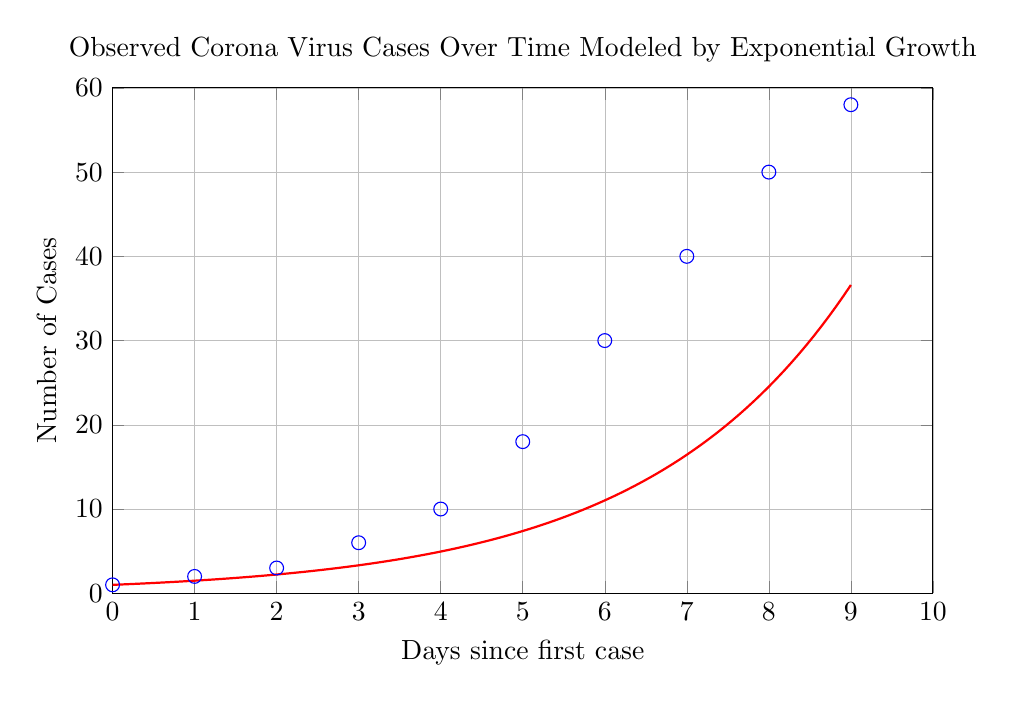
\begin{tikzpicture}
\begin{axis}[
    title={Observed Corona Virus Cases Over Time Modeled by Exponential Growth},
    xlabel={Days since first case},
    ylabel={Number of Cases},
    xmin=0, xmax=10,
    ymin=0, ymax=60,
    grid=both,
    major grid style={line width=.2pt,draw=gray!50},
    minor grid style={line width=.1pt,draw=gray!20},
    width=12cm,
    height=8cm,
    legend pos=north west,
]

% Example data points (roughly exponential)
\addplot[
    only marks,
    mark=o,
    mark size=2.5pt,
    blue,
] coordinates {
    (0,1) (1,2) (2,3) (3,6) (4,10) (5,18) (6,30) (7,40) (8,50) (9,58)
};
%\addlegendentry{Observed Data}

% Optional: line of best fit (exponential approximation using y = exp(0.4*x))
\addplot[
    red,
    thick,
    domain=0:9,
    samples=100,
] {exp(0.4*x)};
%\addlegendentry{Exponential Approximation}

\end{axis}
\end{tikzpicture}
\vspace{2cm}

Taking the natural logarithm gives a linear relationship:
\[
\ln(I(t)) \approx \lambda t
\]

\medskip


In this activity, we will:

\begin{enumerate}
    \item Run the gradient descent algorithm in an online application.
    \item Record the final estimated value of $\lambda$:
\end{enumerate}

\subsection*{Estimating $R_0$}

The base reproduction number $R_0$ measures how many people, on average, one infected person will infect.

It can be approximated using:
\[
R_0 \approx e^{\lambda T_g}
\]

where $T_g$ is the \textbf{mean generation time} (the average time between infections). For our covid dataset, $T_g \approx 3.5$ days

\medskip




\subsection*{Interpretation}

\begin{itemize}
    \item If $R_0 > 1$: the virus spreads exponentially.
    \item If $R_0 = 1$: the virus remains stable.
    \item If $R_0 < 1$: the virus dies out.
\end{itemize}

\medskip
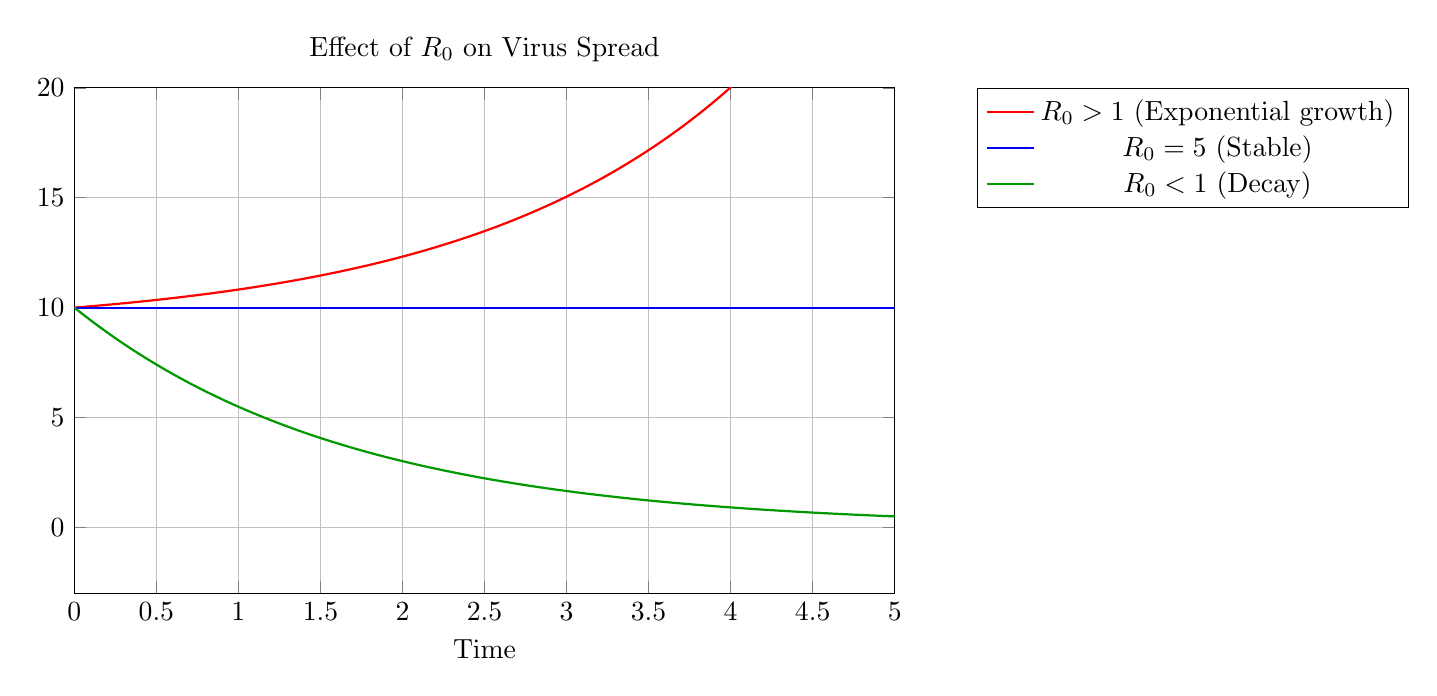
\begin{tikzpicture}
\begin{axis}[
    title={Effect of $R_0$ on Virus Spread},
    xlabel={Time},
    ylabel={},
    xmin=0, xmax=5,
    ymin=-3, ymax=20,
    grid=both,
    width=12cm,
    height=8cm,
    legend style={
        at={(1.1,1)},
        anchor=north west,
        fill=white,
        draw=black
    },
]

% R0 > 1 (growth)
\addplot[
    red,
    thick,
    domain=0:5,
    samples=100,
] {exp(0.6*x) + 9};
\addlegendentry{$R_0 > 1$ (Exponential growth)}

% R0 = 1 (constant)
\addplot[
    blue,
    thick,
    domain=0:5,
] {10};
\addlegendentry{$R_0 = 5$ (Stable)}

% R0 < 1 (decay)
\addplot[
    green!60!black,
    thick,
    domain=0:5,
    samples=100,
] {10*exp(-0.6*x)};
\addlegendentry{$R_0 < 1$ (Decay)}

\end{axis}
\end{tikzpicture}

\vspace{0.5cm}



%\newpage
Use this link \href{https://woodword0-gradientdescentapplication2.hf.space/}{Open the Gradient Descent App} to answer the following questions:
\begin{enumerate}
\item First start with any fixed guess for $\lambda$, $\alpha$ and the number of steps. You can see how well the line $\lambda t$ approximates the dataset in the first graph ``Initial Model vs Data." Click the ``Run Gradient Descent" button to get an estimate for the true value of $\lambda$. 
    \begin{enumerate}
    \item[(a)] What value do you get for $\lambda$? 
    {\color{blue}
    Choosing the initial parameters $(\lambda , \alpha , n_{steps}) = (1,0.05,20)$ we get $\lambda \approx 5.0060$
    }
    
    \item[(b)] What is the error of your estimate?
       {\color{blue}
    Choosing the initial parameters $(\lambda , \alpha , n_{steps}) = (1,0.05,20)$ we get an error of  $\approx 10.3315$
    }
    \vspace{3cm}

    \item[(c)] Click the ``Compute $R0$" button. What value did you get for $R0$?
       {\color{blue}
    Choosing the initial parameters $(\lambda , \alpha , n_{steps}) = (1,0.05,20)$ we get $R_0 \approx 1.064$
    }
    \vspace{3cm}

    \item[(d)]  What does this value for $R0$ tell us in the context of this problem?
       {\color{blue}
    With an $R_0$ value of $\approx 1.064$, it appears that the disease will spread exponentially.
    }
    \vspace{3cm}




        \end{enumerate}
%\newpage

\item Now lets try to tune the parameters of the model.
\begin{enumerate}
\item[(a)] Now keep $\alpha$ the same as before but change the number of steps to 50. How does changing the number of steps affect the error?
{\color{blue}
    Choosing the initial parameters $(\lambda , \alpha , n_{steps}) = (1,0.05,50)$ we get an error of $\approx 5.7234$. So, the error went down when we increased the number of steps to 50.
    }
\vspace{4cm}

\item[(b)] Now keep the number of steps as before  and change $\alpha$ to 0.01. How does changing the learning rate affect the error?
{\color{blue}
    Choosing the initial parameters $(\lambda , \alpha , n_{steps}) = (1,0.01,20)$ we get an error of $\approx 5.7234$. So, the error went up (got worse) when we decreased the learning rate to $\alpha = 0.01$.
    }
\vspace{4cm}

\item[(c)] Use your observations to find an initial value for $\lambda$ and for $\alpha$ and try to get the smallest error you can using the least number of steps possible.
{\color{blue}
    Choosing the initial parameters $(\lambda , \alpha , n_{steps}) = (8.87,0.01,1)$ we can minimize the error at $\approx 5.1029$. By playing with the algorithm and making an educated guess for lambda, we can minimize computing time.
    }
\vspace{4cm}



\end{enumerate}
\vspace{4cm}



%\newpage

\item Finally, you have tuned your model.
    \begin{enumerate}
    \item[(a)] What inital value did you choose for  $\lambda$? \\
    {\color{blue}
    $\lambda = 8.87$. 
    }
    \vspace{3cm}
    
    \item[(b)] What value do you get for the approximated $\lambda$?\\ 
    {\color{blue}
    Choosing the initial parameters $(\lambda , \alpha , n_{steps}) = (8.87,0.01,1)$ we can minimize the error at $\lambda \approx 8.8700$. 
    }
    \vspace{3cm}
    
    \item[(c)] How many steps did your model need to converge to the minimal error?\\
    {\color{blue} Just one step!}
    \vspace{3cm}
    
    \item[(d)] What value do you get for $R0$? \\
    {\color{blue} For this configuration of the model, $R_0 \approx 1.116$}
    \vspace{3cm}
    
    \item[(e)] What is the error of your estimate?\\
    {\color{blue} The error is $\approx 5.1029$}
    \vspace{3cm}

    \end{enumerate}




    
\newpage
\item An epidemiologist at the National Institutes of Health is preparing a grant proposal to request emergency funding in response to a viral outbreak. Rather than making a simple yes/no recommendation, they must estimate how much funding will be needed based on projected disease spread.


Assume:
\begin{enumerate}
    \item Each infected individual costs the healthcare system \$10{,}000 on average.
    \item Each \$100{,}000 of preventative measures (funded by the grant) can reduce the effective reproduction number by 5\%.
\end{enumerate}
    \vspace{0.5cm}

\begin{enumerate}
    \item[(a)]  Using your estimated value of $R_0$, project the average number people that 1{,}000 people will infect.\\
{\color{blue}
$1000 \times 1.116 = 1116$ cases.
}
        \vspace{3cm}

    \item[(b)]  Estimate the average number people that 1{,}000 people will infect if the grant is funded and $R_0$ is reduced by 5\%.\\
{\color{blue}
$1000 \times 1.116*(1 - 0.05) = 1060.2$ cases.
}
        \vspace{3cm}

    \item[(c)]  If each infected individual costs the healthcare system \$10{,}000 on average, calculate the total cost savings  for 1{,}000 people due to intervention.\\
{\color{blue}
$1116 - 1060.2 = 55.8 \cdot \$10{,}000 = 558{,}000$.
}
        \vspace{3cm}

    \item[(d)] How much funding would be required to stabilize the virus?
{\color{blue}
 $1.116(1 - 0.05)^n = 1 \implies (0.95)^n = \frac{1}{1.116} \implies n \approx  \frac{-\ln(1.116)}{\ln(0.95)} \approx 2.13967 \approx 2.14$.
 Funding Required = $2.14 \times 100{,}000 = 214{,}000$. Since funding is given in \$100{,}000 increments, to ensure the outbreak is contained, we recommend requesting at least \$300{,}000 in funding, as smaller amounts will not reduce transmission below the critical threshold. If no funding is requested, the outbreak will continue to grow, leading to exponentially increasing infections and significantly higher long-term costs.
}   
\vspace{3cm}


\end{enumerate}

\end{enumerate}

\end{document}
\begin{enumerate}
Answer the following questions.

\begin{enumerate}
\item First start with a linear function from the drop down menu and set the learning rate to $alpha = 0.1$. Run the gradient descent for 20 steps. Record the values for $w$ and $b$ below and test your parameters. What is the error?
\vspace{4cm}

\item Now keep $\alpha$ the same as before but change the number of steps to 50. How did increasing the number of steps affect the error?
\vspace{4cm}

\item Change the number of steps back to 20 and change $\alpha$ to 0.01. How did decreasing the learning rate affect the error?
\vspace{4cm}

\item Do you think this is giving you a good approximation of the data?
\vspace{4cm}


\item How could you improve this approximation?
\end{enumerate}
%\newpage

\begin{enumerate}
\item Now select the logarithmic activation function from the drop down menu and set the learning rate to $alpha = 0.1$. Run the gradient descent for 20 steps. Record the values for $w$ and $b$ below and test your parameters. What is the error?
\vspace{4cm}

\item Now keep $\alpha$ the same as before but change the number of steps to 50. How did increasing the number of steps affect the error?
\vspace{4cm}

\item Change the number of steps back to 20 and change $\alpha$ to 0.01. How did decreasing the learning rate affect the error?
\vspace{4cm}

\item Do you think this is giving you a good approximation of the data?
\vspace{4cm}


\item How could you improve this approximation?
\end{enumerate}
\newpage

\begin{enumerate}
\item Now select the exponential activation function from the drop down menu and set the learning rate to $alpha = 0.1$. Run the gradient descent for 20 steps. Record the values for $w$ and $b$ below and test your parameters. What is the error?
\vspace{4cm}

\item Now keep $\alpha$ the same as before but change the number of steps to 50. How did increasing the number of steps affect the error?
\vspace{4cm}

\item Change the number of steps back to 20 and change $\alpha$ to 0.01. How did decreasing the learning rate affect the error?
\vspace{4cm}

\item Do you think this is giving you a good approximation of the data?
\vspace{4cm}


\item How could you improve this approximation?
\end{enumerate}
\newpage

\begin{enumerate}
    \item Select one function and by manipulating the learning rate and number of steps do your best to find the $w$ and $b$ that gives the lowest possible error. 
    \vspace{4cm}
    
    \item Write an expression for your activation function using the $w$ and $b$ that you found.
  \vspace{4cm}
    
    \item What are the units of the domain and range of this function?
      \vspace{4cm}
    \end{enumerate}
\end{enumerate}















































